\section{System} \label{sec:Our System}

\subsection{Operations} \label{sec:kvstore operations}
Our overall system is implemented as a C programming language library and currently exposes the following operations:
    
    \begin{itemize}
        \item \texttt{KVStore\_T KV\_NewKVStore(void);}
        \item \texttt{Bool KV\_Put(KVStore\_T kvStore, KVKey\_T key, const void* value);} %%% update to void in code.
        \item \texttt{const void* KV\_Get(KVStore\_T kvStore, KVKey\_T key);}
    \end{itemize}

\texttt{KV\_NewKVStore} returns a newly created key-value store instance. \texttt{get} retrieves the value associated with the given key in the store. \texttt{put} adds a key-value pair to the key-value store or updates the value associated with an existing key. Our key type \texttt{KVKey\_T} is created from an array of chars with its specified length. The return type of put will be updated to void because put should always succeed, unless perhaps memory allocation fails (which is extremely unlikely).

\subsection{Architecture Overview}

Our system is a client of two internal libraries: a \texttt{B+-tree library} and a \texttt{Bordernode library}. The B+-Tree library enables the creation of B+-Trees and operations on those B+-Trees. The Bordernode library implements a variant of Masstree's \cite{masstree} bordernodes (nodes at the border of two btree layers). See section \ref{sec:B+-tree implementation} for more details. We also implement a \texttt{utility library} for some common definitions and operations used across the different libraries. 

\begin{comment}
    how much detail to go here? 
    
    architecture diagram?
\end{comment}

\subsection{B+-Tree Implementation} \label{sec:B+-tree implementation}


Our system's B+-Tree data structure is similar to the traditional B+-Tree. However, we do not use cross links between leaf nodes in our implementation, but rather add a new independent auxiliary data structure called a B+-Tree cursor. The B+-Tree cursor can be thought of as an array of node pointers and corresponding pointers to entries within each node (Figure \ref{fig:exB+-Tree}). Each entry in an internal node consists of a key and the pointer to its right. The first entry has no key associated with it. It is simply a pointer. In leaf nodes entries consist of keys and pointers to the record/value they are associated with. The first element of the cursor points to an entry in the root node. The second element in the cursor points to an entry in the child of the entry pointed to in the root, and so on until an element of the cursor points to an entry in a leaf node. The cursor therefore points to all the entries (and nodes) in the unique path from an entry in the root to an entry in a leaf node. 

\begin{figure}[h]
    \centering
    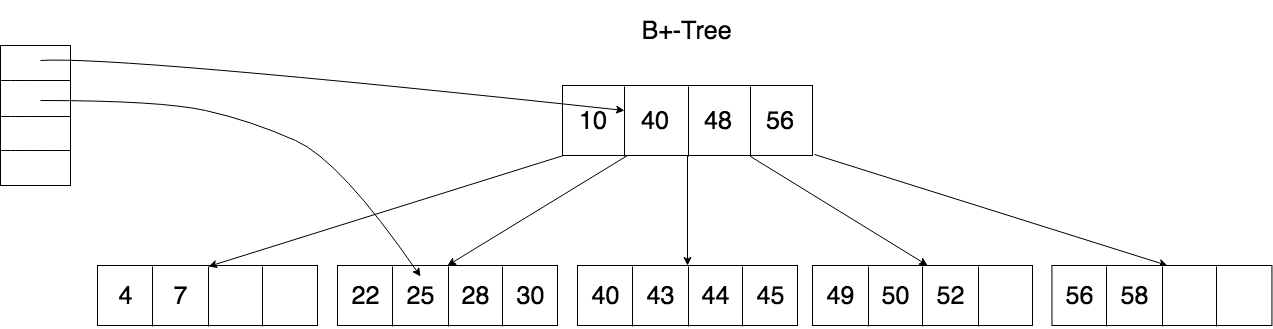
\includegraphics[scale=0.30]{figures/BtreeCursor.png}
    \caption{B+-Tree Cursor Pointing at Key 25.}
    \label{fig:exB+Cursor}
\end{figure}

It is important to know that we were inspired to use this B+Tree with cursor concept from SQLite \cite{SQLite}. SQLite's B-Tree implementation supports both B+-Trees (called B*-Trees in their documentation) and B-Trees. B+-Trees are used as what SQLite calls "Table B-Trees", while B-Trees are used as "Index B-Trees". See \cite{SQLiteFileFormat} for SQLite's database file format documentation. The beauty of this data structure is that it enables \textbf{both} fast sequential gets and puts. More specifically, a sequential get or put operation takes amortized constant time. If these assertions are true, insertion of a set of sorted key-value pairs takes linear time and partially sorting a set of keys involved in a series of get and/or put operations can lead to large performance gains. It would also mean that databases using this B+-Tree scheme can reduce the time it takes for operations that build trees / tables from sorted data e.g. failure recovery, data replication. Moreover, if queries come in batches, they can be partially sorted to reduce processing time. 


\begin{comment}
internal nodes lead search can have high fanout and take relatively less space. makes deletion easier.
cross links guarantee constant time. 

With very large d, All this means we fetch few files when searching for a key or when 

ADD figure of B+-Tree and B-trees and reference it.

Reference insertion and deletion algorithms.

THANK AURELE FOR WORK on this implementation

Draw picture of array and trees.
draw graph of cursor.
Proof of amortized constant time.
refer to both.

2 log n worst case time is what happens in a recursive implementation

examples of building b-tree from sorted or partially-sorted data.

algo for B+-Tree cursor insert.

ubiquitous b-tree - general info about b-trees and variant
modern b-tree techniques = more detailed exploration of b+-trees for database exploration
dbms book - algo for trad b+-trees

figures don't show all details, like other information in nodes / cursor
\end{comment}


\subsubsection {B+-Tree Cursor and Operations}

The B+-Tree Module interface has various methods for operating on B+-Trees, including: \texttt{MoveToFirst}, \texttt{MoveToNext} and \texttt{MoveToPrevious}, However, in this section we will focus on the \texttt{MoveToKey}, \texttt{MoveToNext} and \texttt{PutRecord} operations on B+-Trees with a FANOUT (maximum number of keys per node) of two. The FANOUT can be varied and in our implementation it is set to a default value of 15, similar to the node FANOUT of Masstree \cite{masstree}. 

\begin{figure}[h]
    \centering
    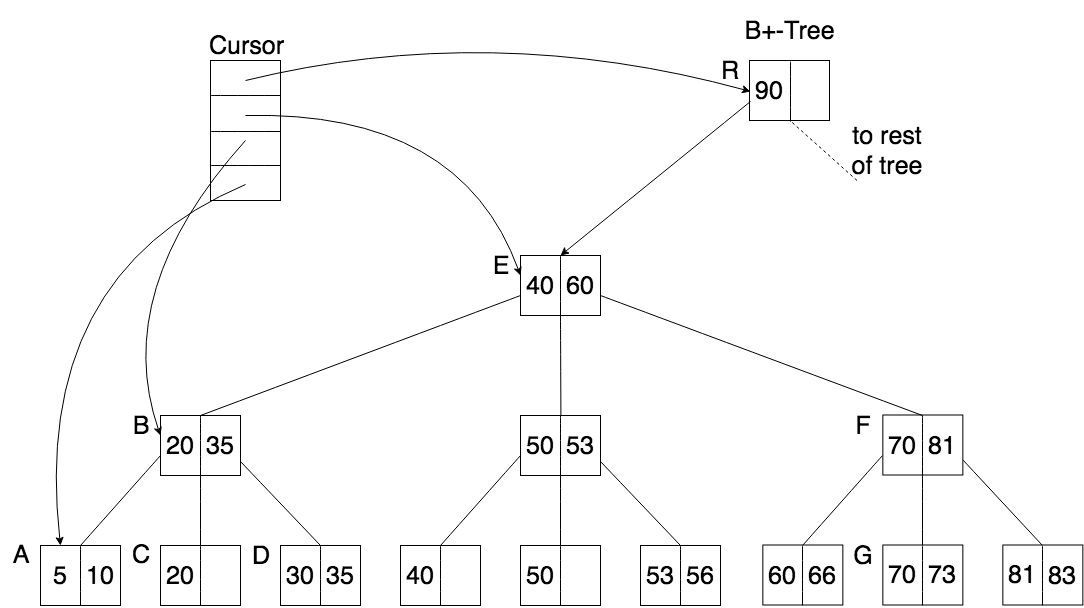
\includegraphics[scale=0.30]{figures/CursorAt5.png}
    \caption{B+-Tree Cursor Pointing at Key 5.}
    \label{fig:exB+Cursor5}
\end{figure}

\texttt{MoveToKey} and \texttt{MoveToKey} operations are simple if the desired key is in the same node. We just search for the correct key within the current node. For example, if the cursor is at key 5 in Figure \ref{fig:exB+Cursor5}, a \texttt{MoveToNext} or \texttt{MoveToKey(10)} operation should simply move the cursor to the next entry in the node, entry 10. However, if the desired key resides in a leaf node one or more nodes away from the current leaf node, there is more work involved. In the traditional implementation of B+-Trees, a move-to-next operation simply uses the cross-links between leaf nodes to get to the next node, and consequently the next key. Nevertheless, a random search always starts from the root. In our B+-Tree implementation a random search (or next operation to an entry in a sibling node) starts from the current leaf node and ascends and descends through the tree \textbf{as needed} to get to the desired key. 

\begin{figure}[h]
    \centering
    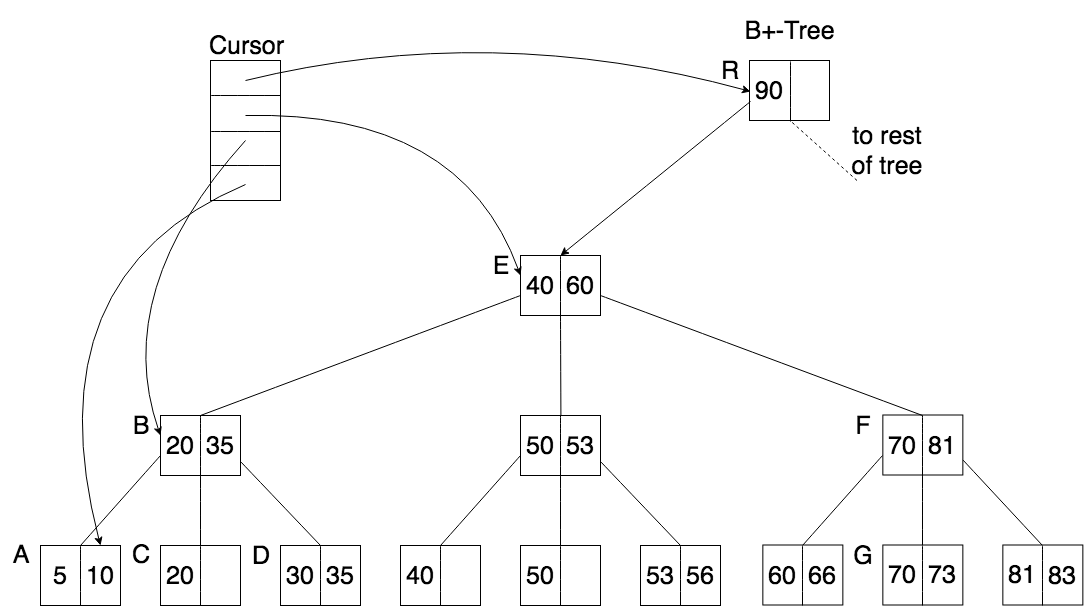
\includegraphics[scale=0.30]{figures/CursorAt10.png}
    \caption{B+-Tree Cursor Pointing at Key 10.}
    \label{fig:exB+Cursor10}
\end{figure}

\begin{figure}[h]
    \centering
    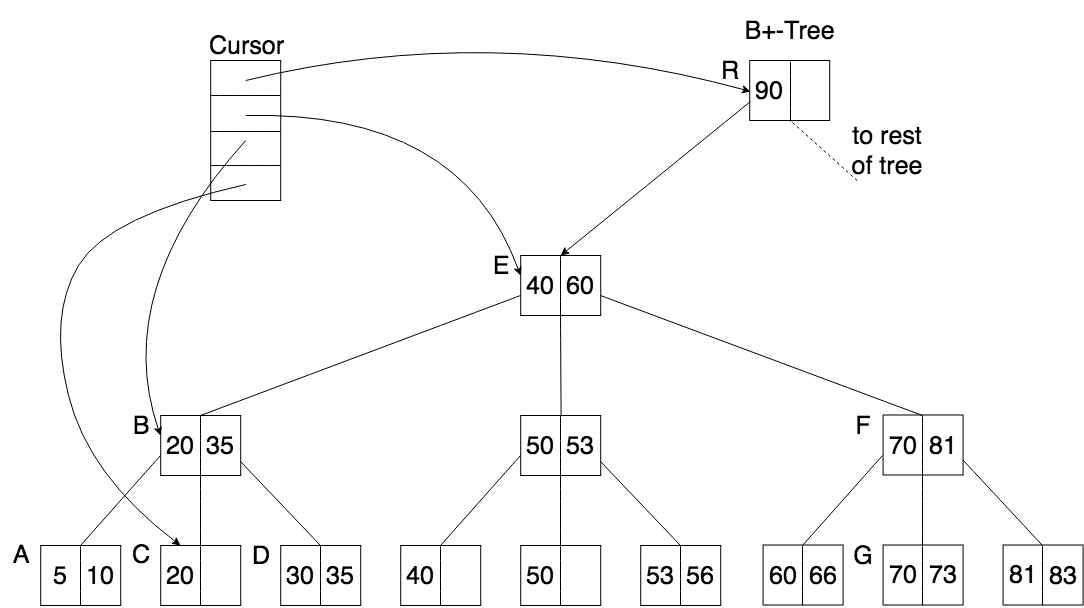
\includegraphics[scale=0.30]{figures/CursorAt20.png}
    \caption{B+-Tree Cursor Pointing at Key 20.}
    \label{fig:exB+Cursor20}
\end{figure}


More specifically, in the case of a \texttt{MoveToNext} operation, the cursor first moves up to the closest ancestor node that it is not pointing to the last entry within. i.e. an ancestor node for which the cursor can move to the next entry within. Afterwards, the cursor then sets the pointer at that level to the next entry in the node and then descends to the entry's smallest leaf child. For example, consider a \texttt{MoveToNext} operation from key 10 (Figure \ref{fig:exB+Cursor10}), this moving the cursor's last pointer from entry 10 on node A to entry 20 on node C (Figure \ref{fig:exB+Cursor20}). To do this, the cursor first ascends to node B. Then it moves its entry pointer for that level to the next entry in node B. Finally it descends to the current entry in node B's smallest leaf child. If the cursor was originally at the last entry in node B, it would have to keep ascending till it either reaches the root or a node where its pointer for that node/level was not previously pointing to the last entry in the node. For example, if the cursor was at key 35 (node D), a move to the next entry (key 40) entails moving up to node E, moving the entry pointer in that node to the next entry and then descending to the left most leaf child.

For a random search, the cursor has to move up to the closest node that is definitely an ancestor of the desired search key. This is a node where the search key is greater than or equal to its first entry and strictly smaller than its last entry. The only exception to this rule is the root. The root is an ancestor of every node in the tree. After a definite ancestor of a key has been found the cursor can then descend down the tree from this node to the desired leaf entry. For example, let the cursor be at key 20 (Figure \ref{fig:exB+Cursor20}). What happens when \texttt{MoveToKey(50)} is called? To move to key 50, the cursor first ascends to node E. It does not go beyond node E as 50 is in between node E's smallest and greatest key. We then descend to node H then node I which contains key 50 (Figure \ref{fig:exB+Cursor20}). What if a call is then made to \texttt{MoveToKey(73)}? In this scenario, the cursor ascends all the way to the root R, and then descends to node E then node F and then node G. The cursor then points at key 73 (Figure \ref{fig:exB+Cursor73}). The cursor has to ascend all the way to node R (the root) because it is impossible from simply looking at node E's entries to know for sure that node E is definitely an ancestor of key 73. All node E's entries can inform us is that children of its greatest entry are greater than or equal to 60. It is possible that another child of E's parent could be the ancestor of key 73. This would be the case if the first key in node R is less than 73. This is an example of the worst case of random search with the B+-Tree scheme. In the worst case, a \texttt{MoveToKey} call takes time proportional to $2 log N$. $log N$ time to ascend to the root and $log N$ time to descend from the root to the apropriate leaf node. This is in contrast to random search in the traditional B+-Tree scheme which always takes time proportional to $log N$. However it is important to note that the cost to ascend will not be significant as most (if not all) of the nodes in the ascend path are likely to be in cache (more specifically higher levels of cache memory) because they have been recently visited. On the other hand, whenever we carry out a random search for a nearby node, we benefit from not needing to ascend to the root and from most of the nodes we visit being in higher levels of cache memory. 

\begin{figure}[h]
    \centering
    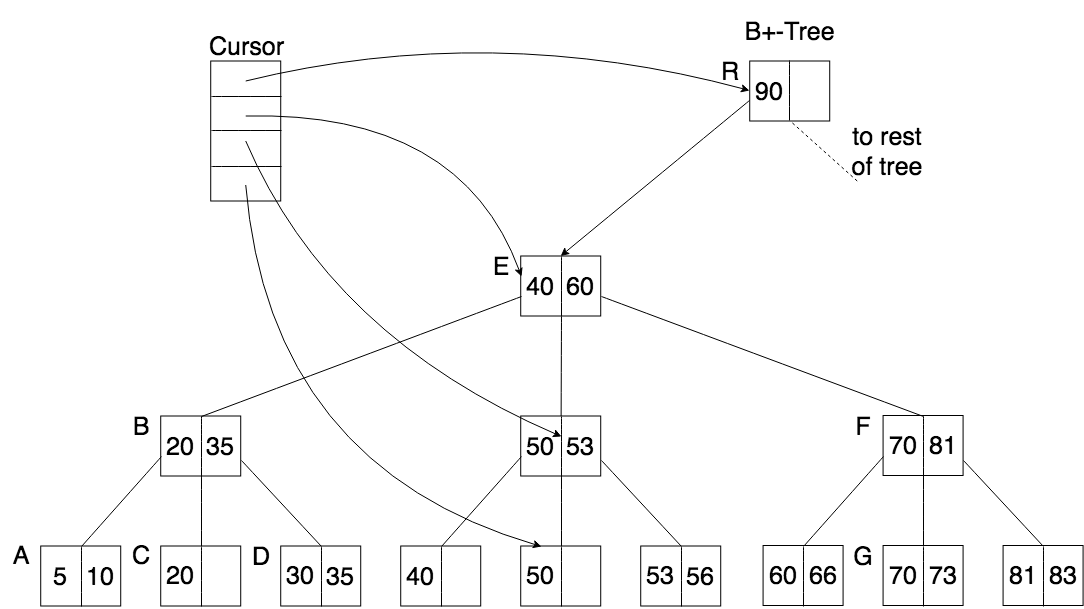
\includegraphics[scale=0.30]{figures/CursorAt50.png}
    \caption{B+-Tree Cursor Pointing at Key 50.}
    \label{fig:exB+Cursor50}
\end{figure}


\begin{figure}[h]
    \centering
    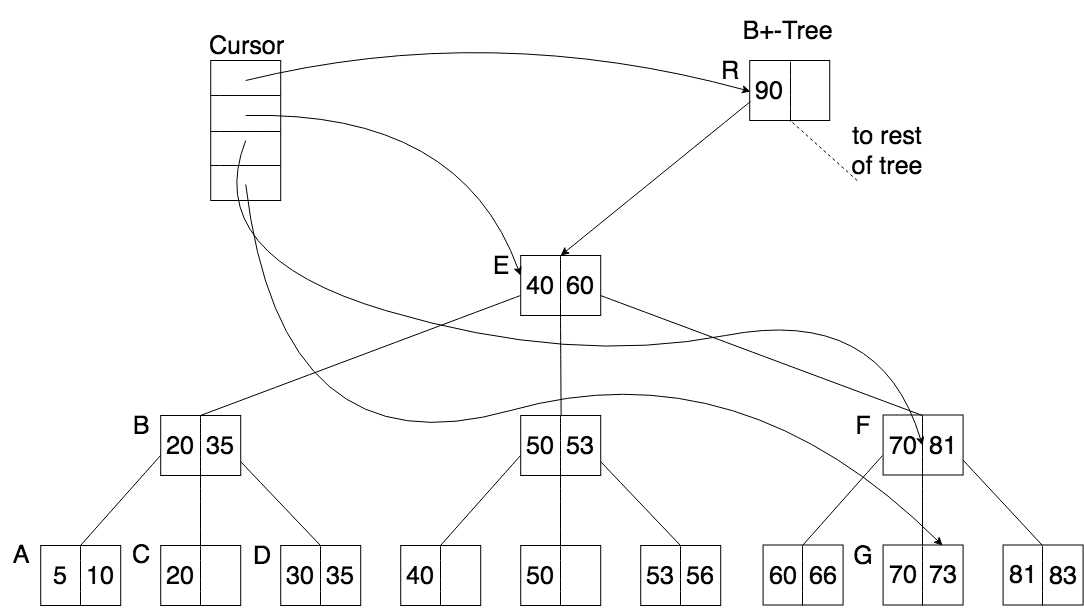
\includegraphics[scale=0.30]{figures/CursorAt73.png}
    \caption{B+-Tree Cursor Pointing at Key 73.}
    \label{fig:exB+Cursor73}
\end{figure}


Sequential (next) operations are fast as well. Most of the time they entail simply moving to the next element in a node, a few times they entail a jump from a node to its right sibling node which often involves fewer node accesses and occasionally, in the worst case, involves $2h$ node accesses, where $h$ is the height of the tree. Inserts can benefit from using this scheme (i.e using a cursor that remembers its current location and the path to it). With sequential inserts, most of the time, the current node has enough space for the next key. Sometimes, we need to split the node (node splits are described briefly in \ref{sec:indexB+-trees}). Most of the time, a single split is enough. Sometimes the split propagates upward to one or more nodes. Occasionally, a node split propagates up multiple levels. As a result, we expect that a sequential put or random put \textbf{near} the cursor's current location will be quick and simply involves the cost of moving to a nearby location and inserting a key; both of these steps (move and put) are often fast if the key to be put into the tree is near the key the cursor is pointing to.

\begin{comment}
   Nevertheless, it is unlikely that, in a series of random searches / move-to-key calls, the desired key is always very far from the cursor's current position. Sure, except due to caching doing this constantly is very fast.
\end{comment}
 
 

In conclusion, aside from reducing the number of node accesses needed in move and put operations, the B+-Tree with cursor scheme benefits highly from cache-locality when the cursor does not move too far. It is less likely to access unnecessary nodes in the path from parent to the desired key, rather it is more likely to revisit previously visited nodes. For example, when traversing the tree from keys 5 to 35 (imagine a range query or sequential updates), our B+-Tree with cursor scheme visits only nodes A, B, C and D. Note we visit node B FANOUT (two) times. This implies that if a sequence of operations is partially sorted by key we can experience massive performance gains, subject to how much we sort the sequence of operations. It is important to note that SQLite \cite{SQLite} (which uses this B+-Tree with cursor scheme) does not always benefit if the cursor is at a key close to a search key. Indeed, SQLite's \texttt{sqlite3BtreeNext} function behaves similarly to our \texttt{MoveToNext} function: most of the time the next key would be in the current node and SQLite's cursors only ascends the tree as needed. Nevertheless, SQLite's \texttt{MoveTo} function always starts searching for the desired key from the root, unless the cursor is already at the correct position. This is in contrast to our implementation of \texttt{MoveToKey} which never begins search from the root. Therefore, a partially random sequence of operations would be expected to execute as quickly as a random sequence of operations and experience no performance gains in SQLite. 

\subsubsection {Why Sequential Operations are Amortized Constant Time}

\begin{figure}[h]
    \centering
    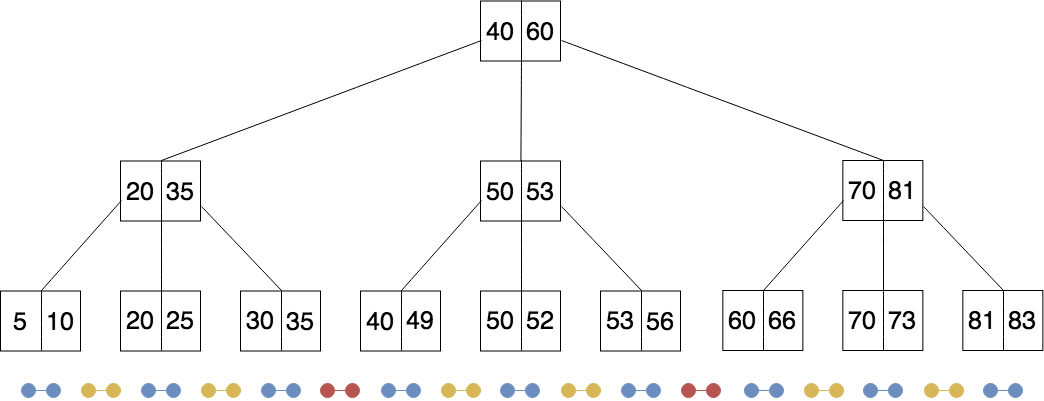
\includegraphics[scale=0.30]{figures/amortizedtimenextexample.png}
    \caption{Example B+-Tree with 18 keys and height 3 (cursor not shown). When sequentially visiting all keys in the B+-Tree, there are 17 total next operations: 9 blue next operations, 6 yellow next operations and 2 red next operations.}
    \label{fig:amortizedanalysisheight3}
\end{figure}


In this section, we will investigate the claim made in \ref{sec:indexB+-trees} that a sequential get or put operation takes amortized constant time. Figure \ref{fig:amortizedanalysisheight3} gives an intuition for why this might be the case. Traversing through the tree in Figure \ref{fig:amortizedanalysisheight3} from key 5 to key 83 takes 17 next operations. Most (about half) of these  operations are the low cost blue next operations.These blue next operations cost little as they simply involve moving the cursor to the next element in the node and involve zero extra node accesses. The other (roughly) half of next operations require a jump from one node to another. Most of these next operations require the cursor moving up only one level and then down to reach the sibling node containing the next entry. These are the yellow operations which require only two node accesses. Few of these next operations require the cursor moving up to the root and then down to the next entry in the sibling node. These are the red next operations, the most costly next operations.



\begin{figure}[p]
    \centering
    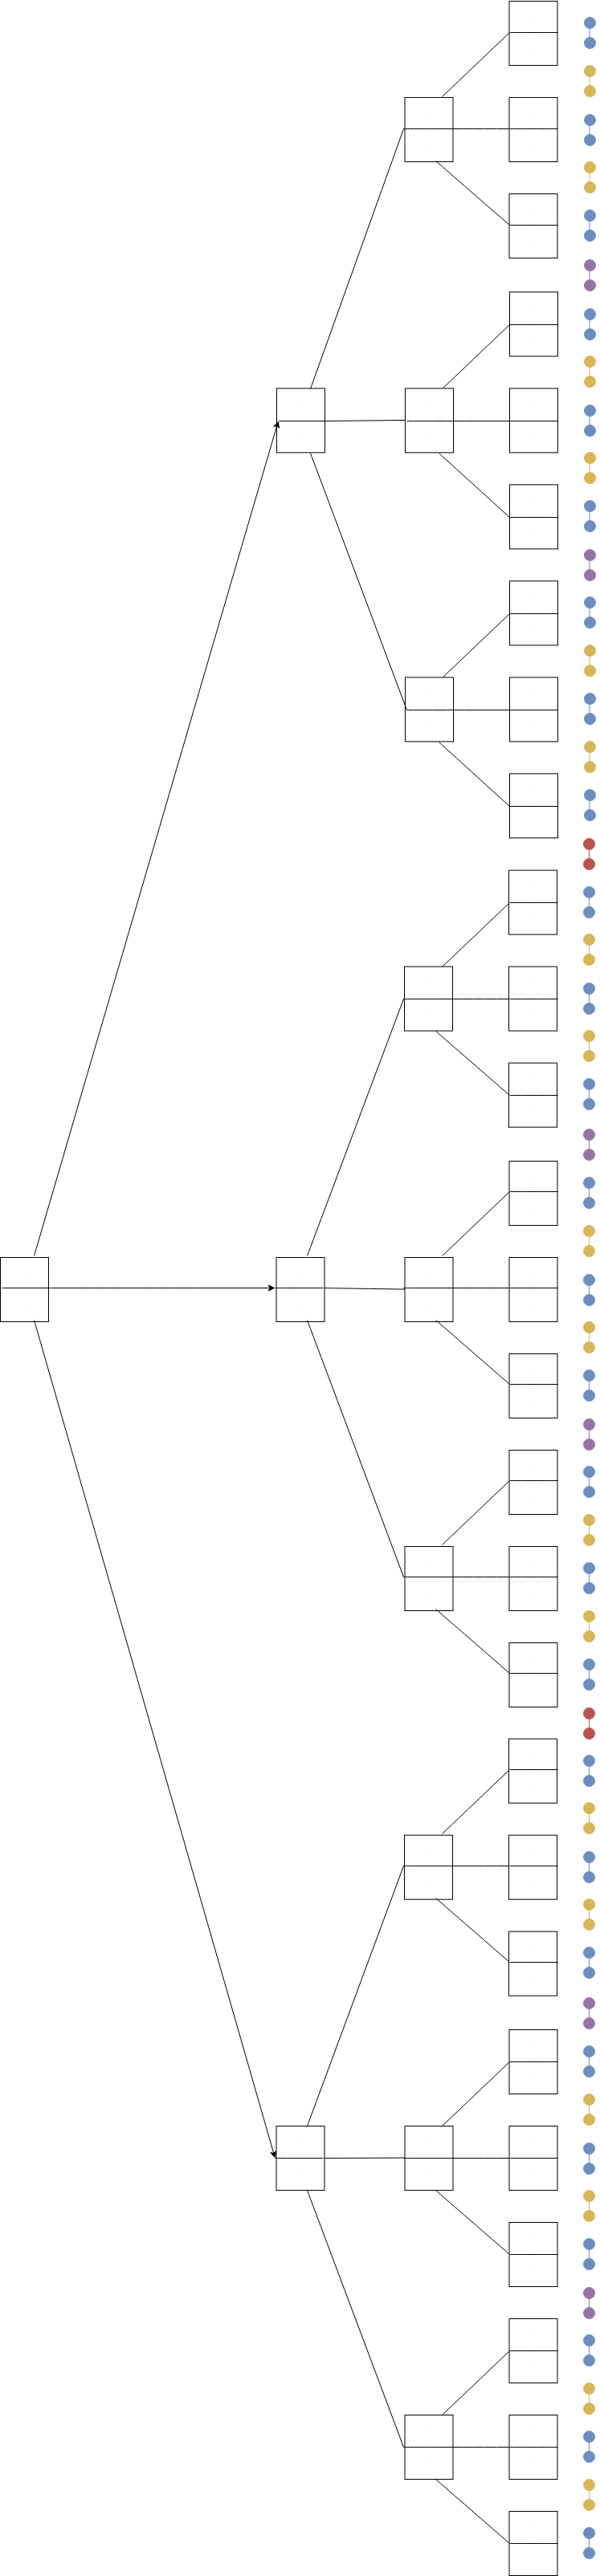
\includegraphics[scale=0.18]{figures/amortizedtimenextexamplehugerotated.png}
    \caption{Example B+-Tree with 54 keys and height 4 (cursor not shown). When sequentially visiting all keys in the B+-Tree, there are 53 total next operations: 27 blue next operations, 18 yellow next operations, 6 purple operations and 2 red next operations.}
    \label{fig:amortizedanalysisheight4}
\end{figure}

For our tree with 18 keys, in order of costliness there are:

    \begin{itemize}
        \item 2 red operations
        \item 6 yellow operations
        \item 9 blue operations
    \end{itemize}

If our tree was a level deeper, as in Figure \ref{fig:amortizedanalysisheight4}, in order of costliness there are:

    \begin{itemize}
        \item 2 red operations
        \item 6 purple operations
        \item 18 yellow operations
        \item 27 blue operations
    \end{itemize}
    
We see that the most costly jumps occur $2 * 3^0$ times, the next most costly operations occur $2 * 3^1$, the next most costly operations occur $2 * 3^2$ times and so on. The least costly operations, however, occur $3^h$ times where $h$ = the height (number of levels) of the tree. This implies that the most costly operations which are proportional to $log N$ where $N$ is the number of entries in the tree occur very infrequently. If each next operation was logarithmic on average, we will expect that most of the next operations are proportional to $log N$. Not only is this not the case, but we see that the more costly an operation, the (exponentially) less likely it is to occur. Put another way, a fraction of the time a next operation requires that we jump to the next node.  When jumping from a node to the next, a majority of the time moving up one level and then back down is sufficient. A fraction of the time when we jump between two nodes, we need to move up two levels and then back down. An even smaller fraction of the time we need to move up three levels and then back down, and so on and so forth.  

With this intuition we can find an upper bound of the average cost of a next operation for a tree of any height:

\begin{equation} \label{eq:TnextaveExp1}
    T_{ave} < c + \frac{2}{F} + \frac{4}{F^2} + \frac{6}{F^3} + ... = c + \frac{2 \times 1}{F} + \frac{4 \times 2}{F^2} + \frac{6 \times 3}{F^3} + ...
\end{equation}

\begin{equation} \label{eq:TnextaveSeries}
    T_{ave} < c + \sum_{i=0}^{\infty} \frac{2i}{F^i} 
\end{equation}

where $F$ is the FANOUT - maximum number of keys - in each node in the B+-Tree.


In Equation \ref{eq:TnextaveExp1}, we see that a next operation always takes some constant plus 2 node accesses $\frac{1}{F}$ of the time, plus 4 node accesses $\frac{1}{F^2}$ of the time and so on. The frequency of costly operations decreases exponentially. This is an upper bound because in reality the probability of any jump is $\frac{1}{F}$, low cost and high cost jumps included. So this means that in reality, the most frequent lowest cost jumps occur less than $\frac{1}{F}$ of the time, the next lowest cost jumps occur less than $\frac{1}{F^2}$ of the time and so on. 

The series in equation \ref{eq:TnextaveSeries} is the product of an \textbf{arithmetic} and a \textbf{geometric} series. It is an \textbf{arithmetico-geometric} series. We know that the sum from an arithmetico-geometric series is given by \cite{riley2011foundationmaths}:

\begin{equation} \label{eq:arith-geometricSeries}
    S = \sum_{n=0}^{\infty} (a + n d)r^n = \frac{a}{1-r} + \frac{rd}{(1-r)^2} 
\end{equation}


where $r < 1$.

Equation \ref{eq:TnextaveSeries} can be simplified with \ref{eq:arith-geometricSeries} to yield:

\begin{equation} \label{eq:TnextaveResult}
    T_{ave} < c + \frac{2F}{(F-1)^2} 
\end{equation}


From Equation \ref{eq:TnextaveResult}, we see that the average cost of a next operation for a tree of any height with fanout F is upper-bounded by some small cost plus $\frac{2F}{(F-1)^2}$ node accesses. This shows two things. Firstly, a next operation does not take logarithmic time (is not proportional to the height of the tree), but rather takes amortized constant time. Secondly, the cost of a next operation is inversely proportional to the FANOUT $F$ of the nodes in the tree.

Given the previous analysis, we can also find an upper bound for the cost of a sequential put operation. i.e. a put operation where the key=value pair to be updated or inserted is to be placed beside the current key. We know that the cost of a sequential put operation is the cost to move to the appropriate node (same node or sibling node) plus the cost of inserting the entry. We already know that the cost to move to the next key (next appropriate node) is less than the upper bound in Equation \ref{eq:TnextaveResult}. We know that inserting a key-value pair in a node takes some constant and might involve node splits. How often are node splits? Imagine a sequence of sequential inserts, where each key is not present in the tree. Most of the time a node will have space for an insert and not require any node splits (see \ref{sec:indexB+-trees}). A fraction of the time (proportional to $\frac{1}{F}$) there is a node split. A fraction of the time when there is a node split it propagates up to the next level, a fraction of the time when a split propagates by one extra level it propagates another level, and so on.  

We can find the average cost to insert a new key into a node by simplifying the following inequality:

\begin{equation} \label{eq:TinsertAtLocation}
    T_{ins} < c + c_{split}(\frac{1}{F} + \frac{2}{F^2} + \frac{3}{F^3} + ...)
\end{equation}

That is the cost of inserting a new key-value pair is less than some constant plus the cost of a split that occurs at most some time proportional to $\frac{1}{F}$ plus the cost of two splits that occurs at most some time proportional to $\frac{1}{F^2}$ and so on. The constant$c_{split}$ is to account for the fact that splits occur in proportion to the fractions involved in the geometric series.

\begin{equation} \label{eq:TinsertAtLocationResult}
    T_{ins} < c + c_{split}\sum_{i=0}^{\infty} \frac{i}{F^i} = c + \frac{c_{split}F}{(F-1)^2} 
\end{equation}

Using Equation \ref{eq:arith-geometricSeries} we solve the arithmetico-geometric series in Equation \ref{eq:TinsertAtLocation} to find an upper bound on the cost of insertions.

Putting equation \ref{eq:TnextaveResult} and equation \ref{eq:TinsertAtLocationResult} together an upper bound on the cost of a sequential insert and, consequently, a sequential put is:

\begin{equation} \label{eq:Tseqput}
    T_{seqput} < T_{ins} + T_{ave} = c_1 + \frac{2F}{(F-1)^2} + c_2 + \frac{c_{split}F}{(F-1)^2} 
\end{equation}


As we can see from equation \ref{eq:Tseqput}, the time it takes for a sequential put is lest than some constant inversely proportional to the fanout $F$. Therefore sequential puts also take amortized constant time. 

\begin{comment}
If we have d to the (h) keys, in the best case next takes constant time, in the worst case it take time proportional to h, as we have to go to the root and back down. however, if we have n random gets or get next operations this happens once every n times.
\end{comment}

\subsection{Key-value Store Implementation} \label{kvstore implementation}

In this section we discuss our key-value store implementation. Our key-value store is implemented in the C programming language as a library (called KVStore). It currently supports the operations outlined in section \ref{sec:kvstore operations}. It is a client of the B+-Tree module \ref{sec:B+-tree implementation} and the BorderNode module. Our B+-Tree module as is can only handle fixed length 8 byte keys. Therefore it must be extended to handle variable length keys. As mentioned in section \ref{sec:VarLCPKeysMasstree}, databases and storage systems that use B+-Trees tend to handle variable length keys by adding a level of indirection between a node's slot array and the record / record key in the node's data area; we also saw how B+-Trees are not optimized for handling keys with long common prefixes. We discussed how Masstree effectively handles variable-length keys and keys with long common prefixes. As a result, our KVStore Module is based on Masstree. It is also a trie-like concatenation of B+-Trees.

\begin{comment}
    For example, in SQLite (where records are stored in files by default), B+-Trees are used as a Table index, while ... index, and each node is a page on disk, variable length keys are .... Other external storage based databases use a similar / different approach (check databasemanagement book and other modern b-tree techniques). With main memory databases there is more flexibility to try different approaches. For example, this system handles variable length keys by this. That system handles variable length keys by that.
    
    Mainmemdbs page 49/52 h-store uses variable sized blocks. modern b-tree techniques indirection vector page 236. 220 database management textbook 220
\end{comment}

\subsubsection{Key-value Store Module and BorderNode Module}

Our key-value store module is based on Masstree. It can be viewed as a serial re-implementation of Masstree. However, there are a few differences. As mentioned previously, it is a client of the B+-Tree module \ref{sec:B+-tree implementation}. We also made the decision to implement border nodes separately from the B+-Tree; our B+-Tree's leaf nodes are not border nodes. Our B+-Tree module's leaf nodes (listing \ref{lst:btreenode}) have fixed length key slices and associated value, but do not have key length fields or key suffixes as in Masstree (see Figure \ref{fig:MasstreenodeDS}). Furthermore, our border nodes contain a key slice, an array of values and a key suffix (listing \ref{lst:bordernode}). Each border node is associated with a key slice and does not have an array of key lengths; key length is implicit in the position of the value in the value array. If there is a key suffix in a bordernode, that means that the 10th key does not have a link to the next layer, and vice versa. 


\begin{lstlisting}[language=C, caption={B+-Tree node type definition}, captionpos=b, label = {lst:btreenode}]

typedef unsigned long Key;

struct Entry {
    Key key;
    Child_or_Record ptr;
};

struct BtNode {
    Bool isLeaf;
    Bool FirstLeaf;
    Bool LastLeaf;
    int numKeys;
    BtNode* ptr0;
    Entry entries[FANOUT];
};
\end{lstlisting}

This design of separating the concept of a bordernode from that of a B+-Tree into two separate modules for use by a key-value store allows for greater modularity. The B+-Tree and BorderNode modules can each easily be replaced with different implementations. It is important to also note that this implementation of Bordernodes use less memory when there are keys with multiple common prefixes. For example, if there are 10 keys with the keyslice "00000000", where each character is a NULL character. In Masstree there would be 10 key slices, 10 values (references) and 10 keylengths. In our scheme, there would be one key slice in the B+-Tree, one reference to a Bordernode pointed to by the entry in the leaf node, 10 values and 4 overhead fields in the Bordernode. In this scenario we use about half the space Masstree uses. However, when every key slice is unique, MassTree has a key slice, a value and a key length associated with each key, while we have a key slice, a border node reference and space for 10 values associated with each key. Note that we can optimize our Bordernode implementation's space usage by removing the keyslice field in the Bordernode and by using a more efficient bordernode implementation when there are only a few keys associated with the bordernode's keyslice. This field is redundant as it will be already present in a B+-Tree entry pointing to the bordernode. 

\begin{lstlisting}[language=C, caption={Border node type definition}, captionpos=b, label={lst:bordernode}]
struct BorderNode {
    unsigned long keySlice;
    void* val[MAX_BN_SIZE];
    size_t keySuffixLength;
    char* keySuffix;
};
\end{lstlisting}

Another difference between our key-value store implementation and Masstree is that in order to leverage the benefits of our B+-Tree with cursor implementations we permanently associate each B+-Tree with a cursor. This is to ensure higher performance when the key involved in the next operation is lexicographically close to the key involved in the previous operation. 
